\documentclass[a4paper]{article} 
\addtolength{\hoffset}{-2.25cm}
\addtolength{\textwidth}{4.5cm}
\addtolength{\voffset}{-3.25cm}
\addtolength{\textheight}{5cm}
\setlength{\parskip}{0pt}
\setlength{\parindent}{0in}

%----------------------------------------------------------------------------------------
%	PACKAGES AND OTHER DOCUMENT CONFIGURATIONS
%----------------------------------------------------------------------------------------

\usepackage[italicdiff]{physics}
%\usepackage{derivative}
\usepackage{tasks}
\usepackage{blindtext} % Package to generate dummy text
\usepackage{charter} % Use the Charter font
\usepackage[utf8]{inputenc} % Use UTF-8 encoding
\usepackage{microtype} % Slightly tweak font spacing for aesthetics
\usepackage[T1]{fontenc}
\usepackage{polski}
\usepackage{enumerate}
\usepackage[utf8]{inputenc}
\usepackage[english, ngerman]{babel} % Language hyphenation and typographical rules
\usepackage{amsthm, amsmath, amssymb} % Mathematical typesetting
\usepackage{float} % Improved interface for floating objects
\usepackage[final, colorlinks = true, 
            linkcolor = black, 
            citecolor = black]{hyperref} % For hyperlinks in the PDF
\usepackage{graphicx, multicol} % Enhanced support for graphics
\usepackage{xcolor} % Driver-independent color extensions
\usepackage{marvosym, wasysym} % More symbols
\usepackage{rotating} % Rotation tools
\usepackage{censor} % Facilities for controlling restricted text
\usepackage{listings, style/lstlisting} % Environment for non-formatted code, !uses style file!
\usepackage{pseudocode} % Environment for specifying algorithms in a natural way
\usepackage{style/avm} % Environment for f-structures, !uses style file!
\usepackage{booktabs} % Enhances quality of tables
\usepackage{tikz-qtree} % Easy tree drawing tool
\tikzset{every tree node/.style={align=center,anchor=north},
         level distance=2cm} % Configuration for q-trees
\usepackage{style/btree} % Configuration for b-trees and b+-trees, !uses style file!
\usepackage[backend=biber,style=numeric,
            sorting=nyt]{biblatex} % Complete reimplementation of bibliographic facilities
\addbibresource{ecl.bib}
\usepackage{csquotes} % Context sensitive quotation facilities
\usepackage[yyyymmdd]{datetime} % Uses YEAR-MONTH-DAY format for dates
\renewcommand{\dateseparator}{-} % Sets dateseparator to '-'
\usepackage{fancyhdr} % Headers and footers
\pagestyle{fancy} % All pages have headers and footers
\fancyhead{}\renewcommand{\headrulewidth}{0pt} % Blank out the default header
\fancyfoot[L]{} % Custom footer text
\fancyfoot[C]{} % Custom footer text
\fancyfoot[R]{\thepage} % Custom footer text
\newcommand{\note}[1]{\marginpar{\scriptsize \textcolor{red}{#1}}} %
\graphicspath{ {./images/} }

%----------------------------------------------------------------------------------------

\begin{document}

%-------------------------------
%	TITLE SECTION
%-------------------------------

\fancyhead[C]{}
\hrule \medskip % Upper rule
\begin{minipage}{0.295\textwidth} 
\raggedright
\footnotesize
Antoni Dąbrowski \hfill\\   
Nr. indeksu 317214\hfill\\
Mail: 317214@uwr.edu.pl
\end{minipage}
\begin{minipage}{0.4\textwidth} 
\centering 
\large 
Statystyka\\ 
\normalsize 
Laboratorium - lista II\\ 
\end{minipage}
\begin{minipage}{0.295\textwidth} 
\raggedleft
\today\hfill\\
\end{minipage}
\medskip\hrule 
\bigskip

%-------------------------------
%	CONTENTS
%-------------------------------


\section{Zadanie pierwsze}
Wygeneruj $n$ obserwacji z rozkładu dwumianowego $b(5,p)$. Na tej podstawie wyznacz wartość estymatora największej wiarygodności wielkości $P(X\geq3)$, gdzie $X\sim b(5,p)$. Doświadczenie powtórz $10000$ razy. Oszacuj wariancję, błąd średniokwadratowy oraz obciążenie analizowanego estymatora. Przedyskutuj uzyskane wyniki w zależności od wyboru parametru $p$.

\subsection{Rozwiązanie}
\textbf{Twierdzenie 1.}
Jeśli $\hat{\theta}$ jest estymatorem największej wiarygodności dla parametru $\theta$, to $f(\hat{\theta})$ jest estymatorem największej wiarygodności dla $f(\theta)$.
\newline

Estymatorem największej wiarygodności parametru $p$ rozkładu dwumianowego $b(n,p)$ jest $\frac{\overline{X}}{n}$, co  pokazywaliśmy na zajęciach. Na mocy powyższego twierdzenia w celu wyznaczenia estymatora największej wiarygodności wartosci $P(X\geq3)={5\choose3}p^3(1-p)^2+{5\choose4}p^4(1-p)+{5\choose5}p^5$ wystarczy w miejsce parametru $p$ wstawić jego estymator.


\begin{table}[H]
\centering
\begin{tabular}{|c|c|c|c|}
\hline
                  & \textbf{wariancja}   & \textbf{błąd średniokwadratowy} & \textbf{obciążenie estymatora} \\ \hline
$n=50,p=0.1$ & 1.6841e-07 & 6.4224e-05 & -0.0080034 \\ \hline
$n=50,p=0.3$ & 0.00013028 & 0.01729409 & -0.1310107 \\ \hline
$n=50,p=0.5$ & 0.00156947 & 0.09761449 & -0.3099113 \\ \hline
$n=50,p=0.7$ & 0.00357802 & 0.09893096 & -0.3087927 \\ \hline
$n=50,p=0.9$ & 0.00076429 & 0.00626934 & -0.0741960 \\ \hline
\end{tabular}
\end{table}

Można zauważyć, że dla skrajnych wartości parametru $p$ uzyskujemy o kilka rzędów wielkości lepsze estymacje niż dla wartości centralnych. Dotyczy to zarówno wariancji, błędu średniokwadratowego jak i obciążenia. Przyczyny szukałbym w wariancji rozkładu dwumianowego - im $p$ jest bliżej połowy, tym większa wariancja.

\section{Zadanie drugie}
Wygeneruj $n$ obserwacji z rozkładu Poissona z parametrem $\lambda$. Na tej podstawie wyznacz wartość estymatora największej wiarygodności wielkości $P(X=x)$, $x=0,1,...,10$, gdzie $X\sim \pi(\lambda)$. Doświadczenie powtórz 10000 razy. Oszacuj wariancję, błąd średniokwadratowy oraz obciążenie analizowanego estymatora. Przedyskutuj wyniki w zależności od wyboru parametru $\lambda$.

\subsection{Rozwiązanie}
Estymatorem największej wiarygodności parametru $\lambda$ rozkładu $Pois(\lambda)$ jest $\overline{X}$, co  pokazywaliśmy na zajęciach. W celu wyznaczenia estymatora największej wiarygodności wartości $P(X=x)=\frac{\lambda^xe^{-\lambda}}{x!}$ wystarczy w miejsce wartości $\lambda$ wstawić jej estymator (Twierdzenie 1.). Dla czytelności i oszczędności miejsca wyniki zaprezentuję na wykresach:
\begin{center}
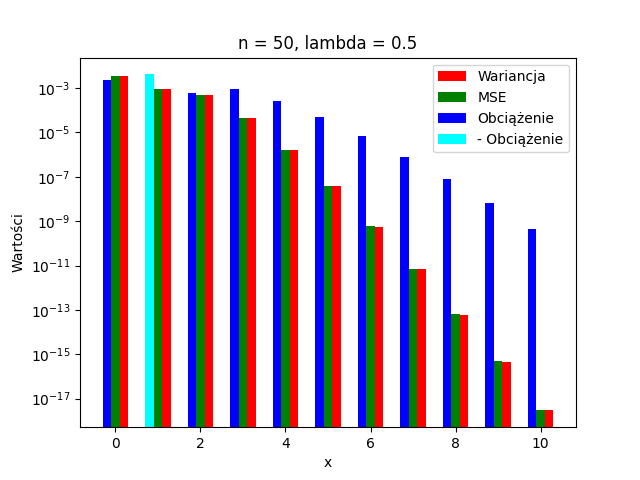
\includegraphics[scale=0.5]{Z2_1}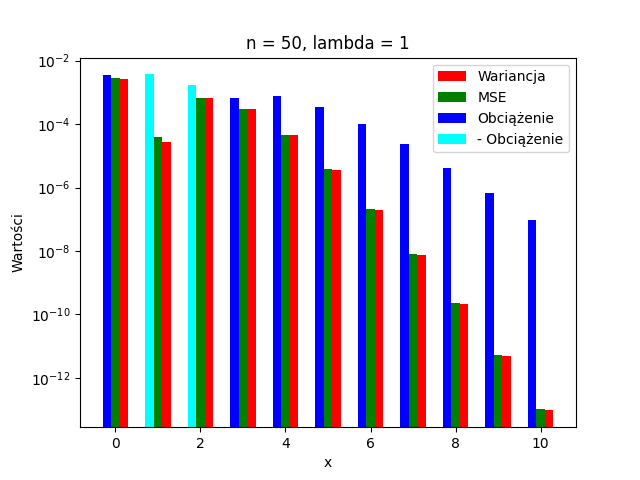
\includegraphics[scale=0.5]{Z2_2}
\end{center}

\begin{center}
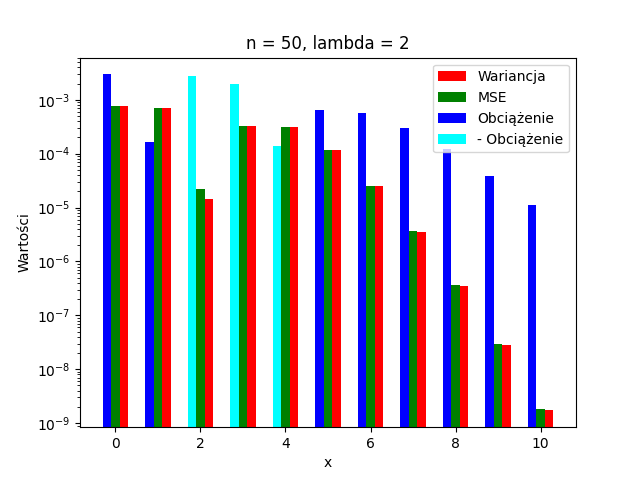
\includegraphics[scale=0.5]{Z2_3}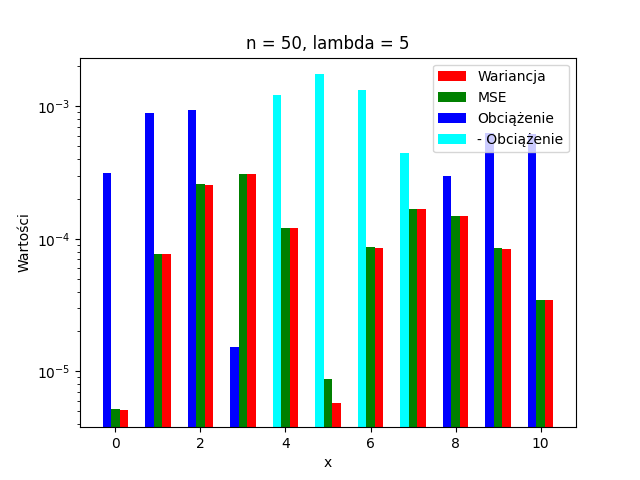
\includegraphics[scale=0.5]{Z2_4} 
\end{center}

Wyniki eksperymentu wskazują na to, że najlepsze estymacje $P(X=x)$ uzyskuje się w najbliższym otoczeniu wartości $\lambda$ oraz przy wartościach bardzo odległych. O ile pierwszego oczekiwałem, to drugiego się nie spodziewałem. Jednak jeśli się przyjrzeć to ma to sens. Dalekie od centrum wartości funkcji gęstości rozkładu lambda są na tyle znikome, że nawet jeśli popełnimy proporcjonalny do nich błąd, to będzie on niezauważalny pod względem wariancji lub MSE.

\section{Zadanie trzecie}
Liczby losowe czy pseudolosowe? Przedyskutuj wybór jednego z określeń na podstawie rozdziału 8.2.1, Koronacki, Mielniczuk (2009), str. 427-429.

\subsection{Rozwiązanie}
Liczby pseudolosowe - liczby generowane deterministycznie przez algorytm symulujący określony rozkład zmiennej losowej. Możliwe jest wielokrotne wylosowanie identycznych liczb w niezależnych eksperymentach jeśli parametry wejściowe algorytmu losującego są takie same. W celu uniknięcia takiego zdarzenia algorytmy pseudolosowe stosowane w programach muszą odnosić się do pewnej zmiennej zewnętrznej wartości np. godziny. Można jednak celowo wielokrotnie symulować eksperyment z takimi samymi danymi losowymi ustawiając określony seed.

\section{Zadanie czwarte}
Wygeneruj $n$ obserwacji z rozkładu beta z parametrami $\theta$ i 1. Doświadczenie powtórz 10000 razy. Na tej podstawie wyznacz wartość estymatora $\widehat{I(\theta)}$ informacji Fishera parametru $\theta$. Wynik zapamiętaj.

Wygeneruj, niezależnie, $n$ obserwacji z rozkładu beta z parametrami $\theta$ i 1. Wyznacz wartość estymatora największej wiarygodności parametru $\theta$. Zdefiniuj nową zmienną $Y = \sqrt{n\widehat{I(\theta)}}(\hat{\theta}-\theta)$. Oblicz jej wartość na podstawie zaobserwowanej próby oraz zapamiętanego wcześniej wyniku.

Doświadczenie powtórz 10000 razy. Narysuj histogram oraz wykres kwantylowo-kwantylowy. Przedyskutuj wybór liczby klas w histogramie oraz sposób wyznaczania kwantyli teoretycznych na wykresie kwantylowo-kwantylowym. Czy rozkład zmiennej losowej $Y$ jest normalny? Odpowiedź uzasadnij.



\subsection{Rozwiązanie}
\textbf{Teoria:}
Dla rozkładu $beta(\theta,1)$ zachodzi własność $\sqrt{n}(\hat{\theta}-\theta)\xrightarrow{\text{D}}N(0,\frac{1}{I(\theta)})$. Jeżeli przemnożymy wyrażenie po lewej przez $\sqrt{\frac{1}{I(\theta)}}$, to asymptotycznie będzie ono zbiegało do standardowego rozkładu normalnego. Stąd asymptotycznie $Y\sim N(0,1)$.
\newline

\textbf{Eksperyment:}
Estymatorem największej wiarygodności parametru $\theta$ rozkładu $beta(\theta,1)$ jest $-\frac{n}{\sum_{i=0}^nx_i}$. Natomiast informacja Fishera dla takiego rozkładu ma postać $\frac{1}{\theta^2}$. Na podstawie 10000 prób estymuję wartość informacji Fishera, następnie w kolejnym eksperymencie traktuję ją jako stałą. Przy wyznaczaniu zmiennej $Y$ jedyną losową wartością jest estymator $\hat{\theta}$.

\begin{center}
$n=50,\theta=0.5$
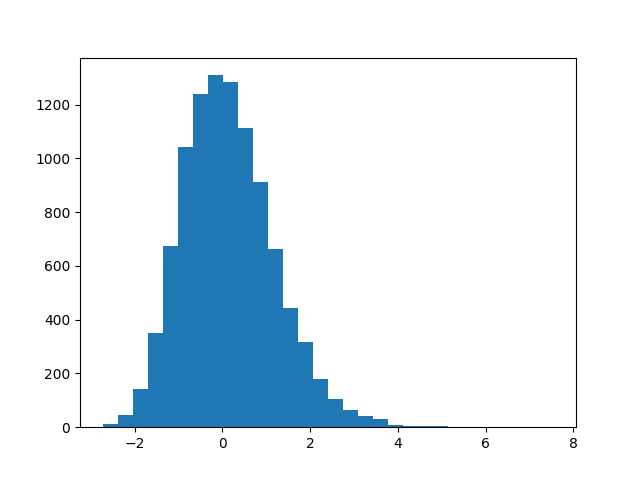
\includegraphics[scale=0.5]{Z4_1a}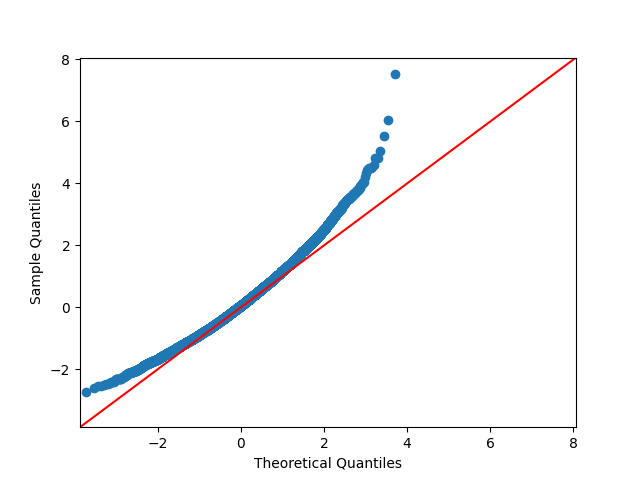
\includegraphics[scale=0.5]{Z4_1b} 
\end{center}


\begin{center}
$n=50,\theta=1$
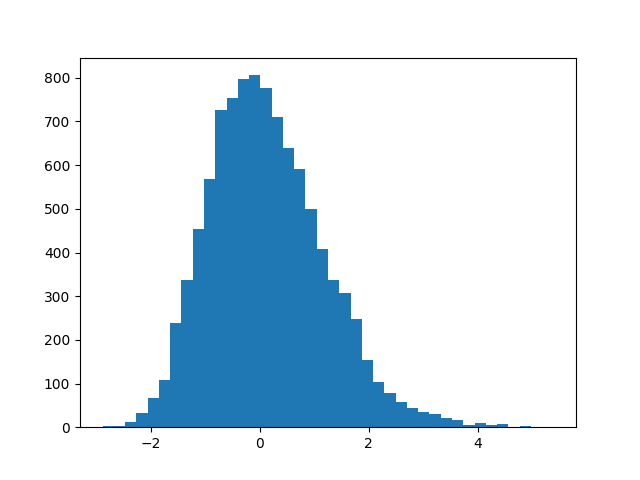
\includegraphics[scale=0.5]{Z4_2a}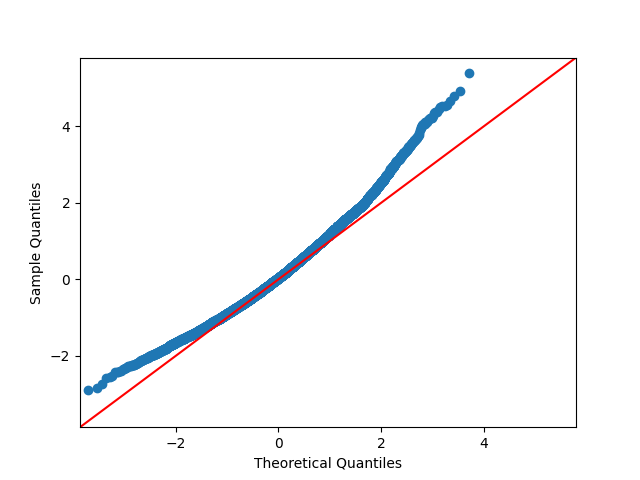
\includegraphics[scale=0.5]{Z4_2b} 
\end{center}
\newpage

\begin{center}
$n=50,\theta=2$
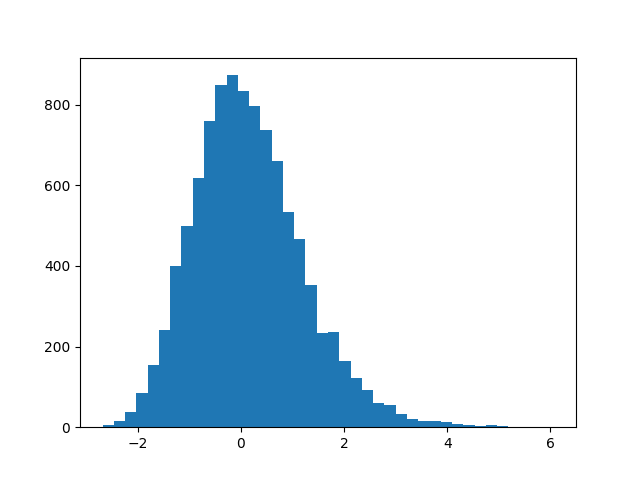
\includegraphics[scale=0.5]{Z4_3a}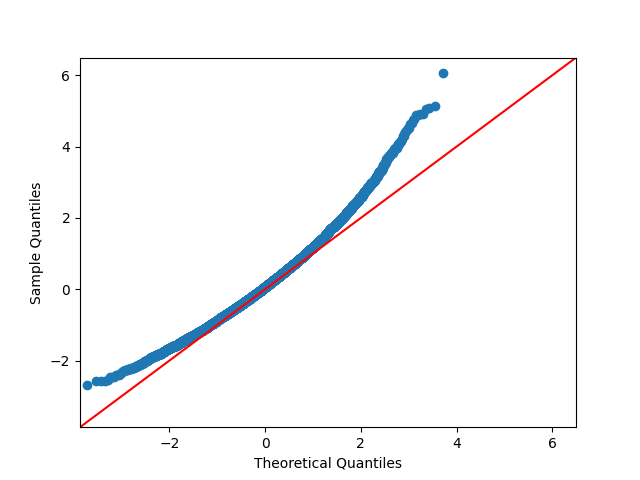
\includegraphics[scale=0.5]{Z4_3b} 
\end{center}

\begin{center}
$n=50,\theta=5$
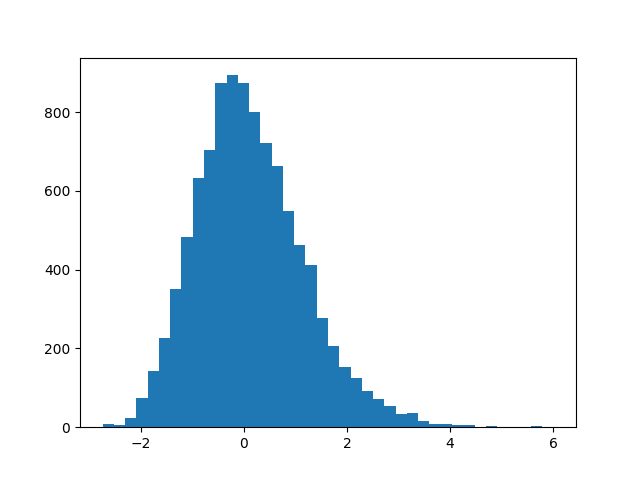
\includegraphics[scale=0.5]{Z4_4a}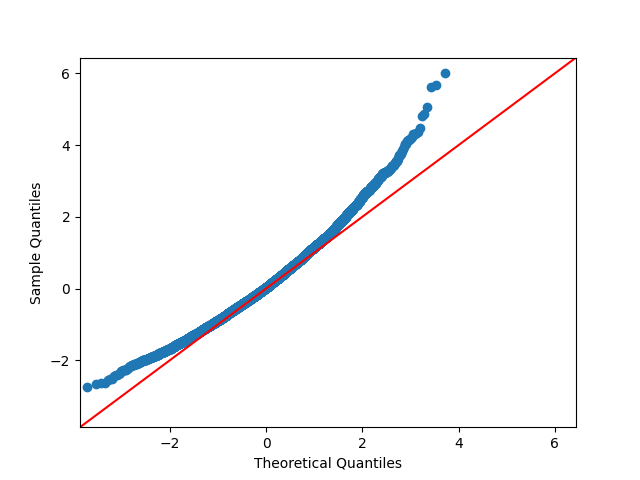
\includegraphics[scale=0.5]{Z4_4b} 
\end{center}


Wykresy po lewej przedstawiają skumulowane dane będące realizacją zmiennej $Y$ pogrupowane na 40 najpopularniejszych klas. Kwantylowo-kwantylowe wykresy po prawej porównują zebrane dane z teoretycznym modelem. Mianowicie sprawdzają czy kwantyle rozkładu $Y$ pokrywają się ze standardowym rozkładem normalnym. Jeśli teoria jest prawdziwa punkty powinny leżeć na czerwonej prostej. Nie dzieje się tak. Obwiniał bym jednak za to nie dość dużą próbę. Gdy testowałem powyższą teorię dla znacznie większego zbioru danych, wówczas jej prawdziwość była widoczna gołym okiem.

\begin{center}
$n=10000,\theta=0.5$
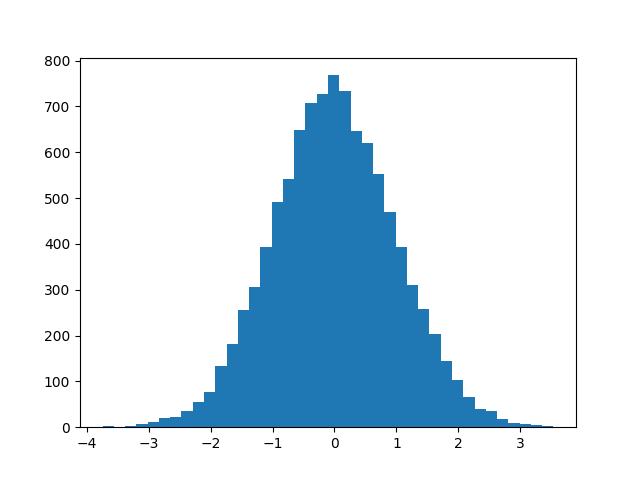
\includegraphics[scale=0.5]{Z4_ok}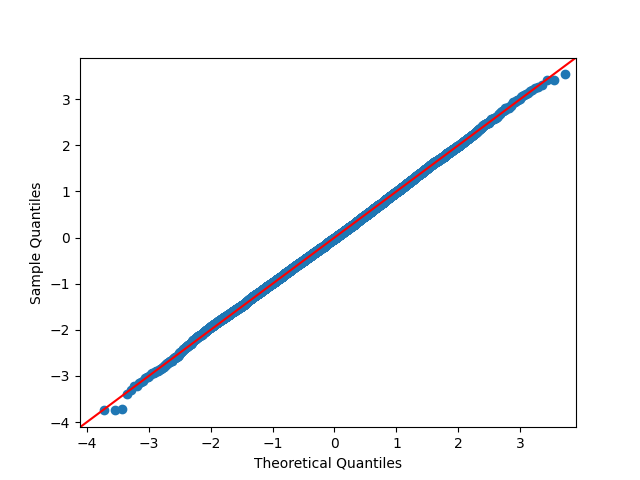
\includegraphics[scale=0.5]{Z4_okb} 
\end{center}

\newpage

\section{Zadanie piąte}
Wygeneruj n obserwacji z rozkładu Laplace'a z parametrem przesunięcia $\theta$ i skali $\sigma$.
\begin{itemize}
	\item $n=50$, $\theta=1$, $\sigma=1$,
	\item $n=50$, $\theta=4$, $\sigma=1$,
	\item $n=50$, $\theta=1$, $\sigma=2$.
\end{itemize}
Na tej podstawie oblicz wartości estymatora parametru $\Theta$ postaci
\begin{itemize}
\item $\hat{\theta}_1 = \bar{X} = (1/n)\sum_{i=1}^nX_i$,
\item $\hat{\theta}_2 = Me\{X_1,...,X_n\},$
\item $\hat{\theta}_3 = \sum_{i=1}^nw_iX_i,\sum_{i=1}^n=1,0\leq w_i\leq 1,i=1,...,n,$ z własnym wyborem wag
\item $\hat{\theta}_4 = \sum_{i=1}^nw_iX_{i:n}, gdzie X_{1:n}\leq\hdots\leq X_{n:n}$ są uporządkowanymi obserwacjami $X_1,...,X_n$,$$w_i=\phi(\Phi^{-1}(\frac{i-1}{n}))-\phi(\Phi^{-1}(\frac{i}{n})),$$ przy czym $\phi$ jest gęstością, a $\Phi$ dystrybuantą standardowego rozkładu normalnego $N(0,1)$.
\end{itemize}
Doświadczenie powtórz $10 000$ razy. Na tej podstawie oszacuj wariancję, błąd średniokwadratowy oraz obciążenie każdego z estymatorów. Przedyskutuj uzyskane wyniki. Który estymator jest optymalny i dlaczego? Skonfrontuj aktualne wyniki z rezultatami uzyskanymi w zadaniu 1 z listy 1.

\subsection{Rozwiązanie}


\begin{table}[H]
\centering
\begin{tabular}{|c|c|c|c|}
\hline
\multicolumn{4}{|c|}{$n=50$, $\theta=1$, $\sigma=1$} \\ \hline
                  & \textbf{wariancja}   & \textbf{błąd średniokwadratowy} & \textbf{obciążenie estymatora} \\ \hline
$\hat{\theta}_1$ & 0.03875034 & 0.03875415 & 0.00195064 \\ \hline
$\hat{\theta}_2$ & 0.02344509 & 0.02344669 & 0.00126500 \\ \hline
$\hat{\theta}_3$ & 0.05080761 & 0.05081367 & 0.00246120 \\ \hline
$\hat{\theta}_4$ & 0.04035669 & 0.15400074 & 0.33711132 \\ \hline
\multicolumn{4}{|c|}{$n=50$, $\theta=4$, $\sigma=1$} \\ \hline
                  & \textbf{wariancja}   & \textbf{błąd średniokwadratowy} & \textbf{obciążenie estymatora} \\ \hline
$\hat{\theta}_1$ & 0.04056163 & 0.04058679 & 0.00501553 \\ \hline
$\hat{\theta}_2$ & 0.02430033 & 0.02430494 & 0.00214645 \\ \hline
$\hat{\theta}_3$ & 0.05324878 & 0.05325972 & 0.00330787 \\ \hline
$\hat{\theta}_4$ & 0.03932861 & 7.14692468 & 2.66600751 \\ \hline
\multicolumn{4}{|c|}{$n=50$, $\theta=1$, $\sigma=2$} \\ \hline
                  & \textbf{wariancja}   & \textbf{błąd średniokwadratowy} & \textbf{obciążenie estymatora} \\ \hline
$\hat{\theta}_1$ & 0.16354358 & 0.16356740 & 0.00488048 \\ \hline
$\hat{\theta}_2$ & 0.10020293 & 0.10020897 & 0.00245707 \\ \hline
$\hat{\theta}_3$ & 0.21412813 & 0.21415132 & 0.00481537 \\ \hline
$\hat{\theta}_4$ & 0.15692464 & 2.95880933 & 1.67388311 \\ \hline
\end{tabular}
\end{table}

Jednoznacznie widać na podstawie eksperymentu, że estymator $\hat{\theta}_2$ jest optymalny. Jest tak ponieważ to właśnie mediana jest estymatorem największej wiarygodności rozkładu Laplace'a. Estymator $\hat{\theta}_4$ podobnie jak na liście pierwszej nie okazał się być skuteczny.
\newline

Uwaga: w przypadku estymatora trzeciego wagi wybieram losowo - w niemal każdym zaobserwowanym przypadku jest to gorsza opcja od stałych wag równych $1/n$

\newpage

\section{Zadanie szóste}
Powtórz eksperyment numeryczny z zadań 1, 2, 4, 5 dla $n=20$ i $n=100$. Przedyskutuj uzyskane rezultaty w nawiązaniu do wcześniejszych wyników.

\subsection{Rozwiązanie}
\textbf{Zadanie 1.}



\begin{table}[H]
\centering
\begin{tabular}{|c|c|c|c|}
\hline
                  & \textbf{wariancja}   & \textbf{błąd średniokwadratowy} & \textbf{obciążenie estymatora} \\ \hline
$n=20,p=0.1$ & 6.7473e-07 & 6.2478e-05 & -0.0078615 \\ \hline
$n=20,p=0.3$ & 0.00036183 & 0.01691975 & -0.1286775 \\ \hline
$n=20,p=0.5$ & 0.00407346 & 0.09788681 & -0.3062896 \\ \hline
$n=20,p=0.7$ & 0.00858359 & 0.10300811 & -0.3072857 \\ \hline
$n=20,p=0.9$ & 0.00191223 & 0.00782896 & -0.0769203 \\ \hline
\end{tabular}
\end{table}
\begin{table}[H]
\centering
\begin{tabular}{|c|c|c|c|}
\hline
                  & \textbf{wariancja}   & \textbf{błąd średniokwadratowy} & \textbf{obciążenie estymatora} \\ \hline
$n=100,p=0.1$ & 7.2515e-08 & 6.4965e-05 & -0.0080556 \\ \hline
$n=100,p=0.3$ & 6.1196e-05 & 0.01738633 & -0.1316250 \\ \hline
$n=100,p=0.5$ & 0.00077864 & 0.09776829 & -0.3114316 \\ \hline
$n=100,p=0.7$ & 0.00173497 & 0.09721602 & -0.3090000 \\ \hline
$n=100,p=0.9$ & 0.00038457 & 0.00584542 & -0.0738975 \\ \hline
\end{tabular}
\end{table}

Dodatkowe obserwacje potwierdzają moje wnioski wysnute w zadaniu pierwszym.
\newline

\textbf{Zadanie 2.}

\begin{center}
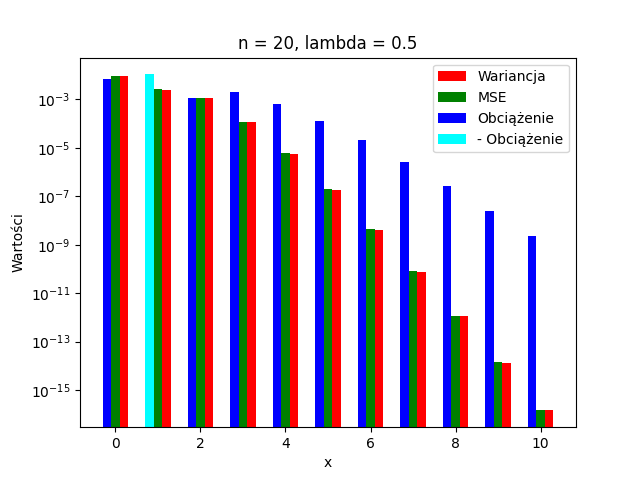
\includegraphics[scale=0.5]{Z6_2_1}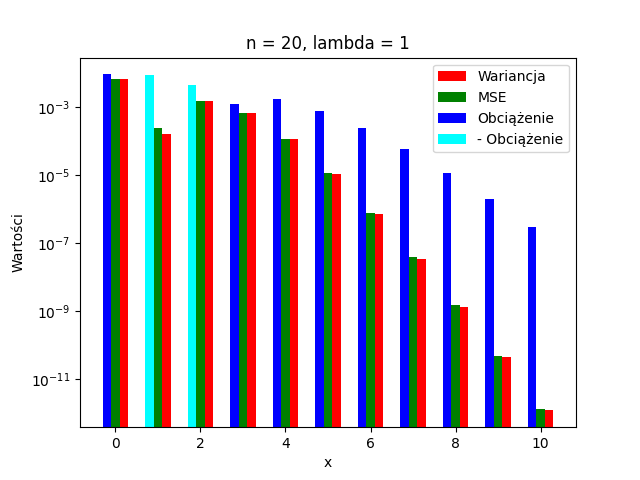
\includegraphics[scale=0.5]{Z6_2_2}
\end{center}

\begin{center}
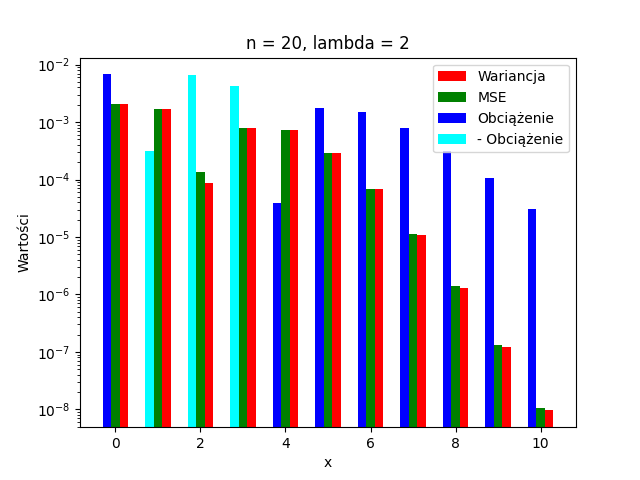
\includegraphics[scale=0.5]{Z6_2_3}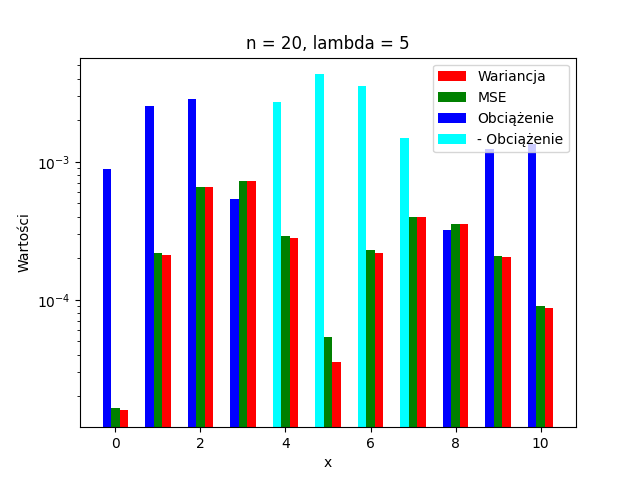
\includegraphics[scale=0.5]{Z6_2_4} 
\end{center}

\begin{center}
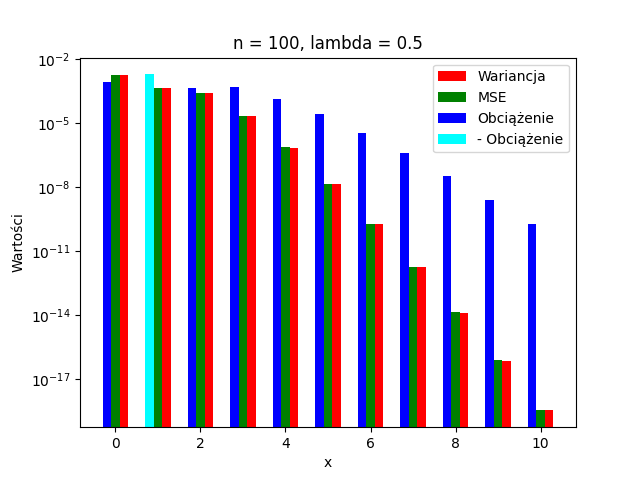
\includegraphics[scale=0.5]{Z6_2_1b}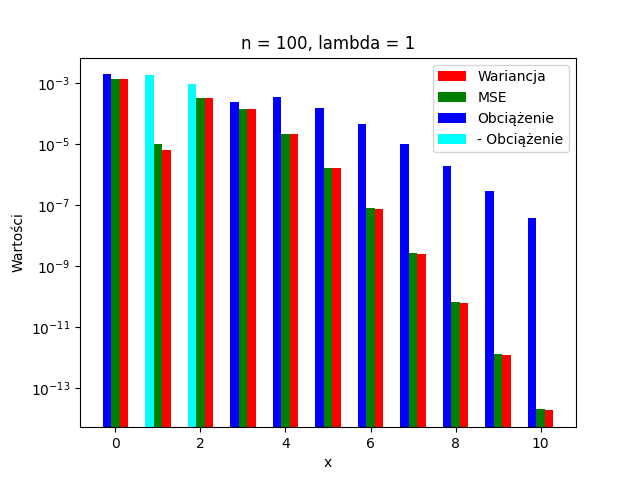
\includegraphics[scale=0.5]{Z6_2_2b}
\end{center}

\begin{center}
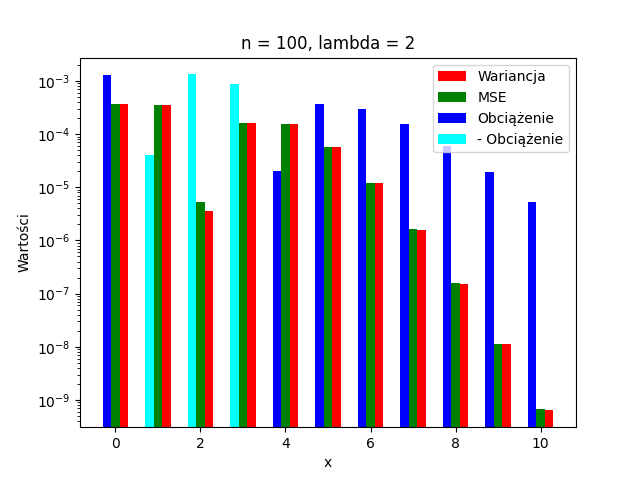
\includegraphics[scale=0.5]{Z6_2_3b}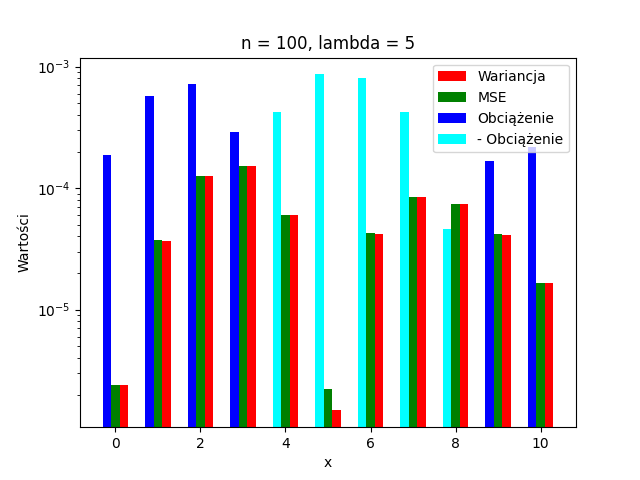
\includegraphics[scale=0.5]{Z6_2_4b} 
\end{center}

Między wykresami dla próbki rzędu 20, 50 oraz 100 widać znikome różnice. Daje to podstawę aby sądzić, że wyniki eksperymentu są dobrym obrazem rzeczywistości, a nie tylko anomalią.
\newline

\textbf{Zadanie 4.}

\begin{center}
$n=20,\theta=0.5$
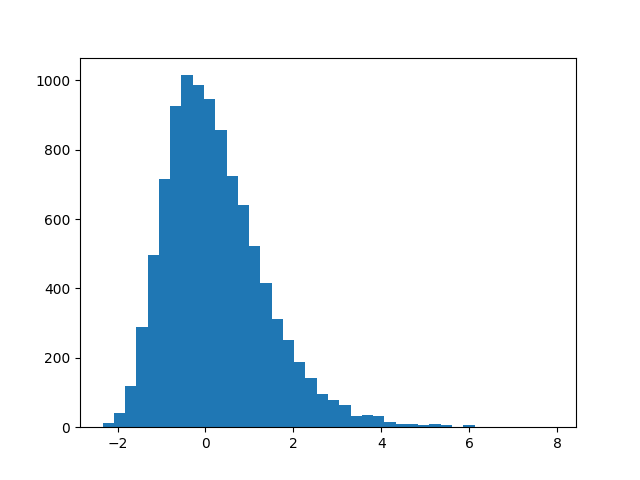
\includegraphics[scale=0.5]{Z6_4_1a}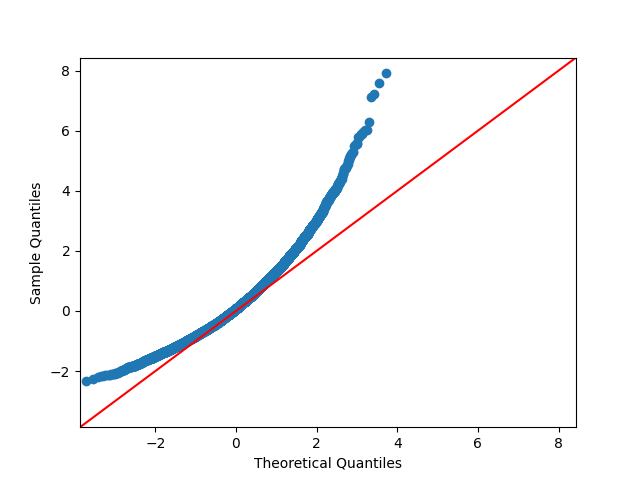
\includegraphics[scale=0.5]{Z6_4_1b} 
\end{center}
\newpage

\begin{center}
$n=20,\theta=1$
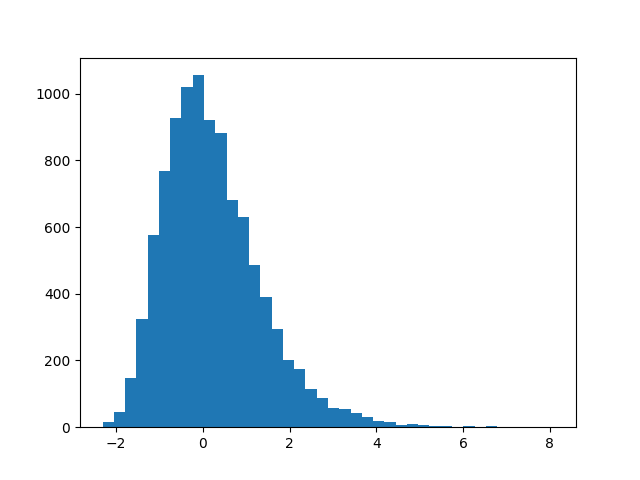
\includegraphics[scale=0.5]{Z6_4_2a}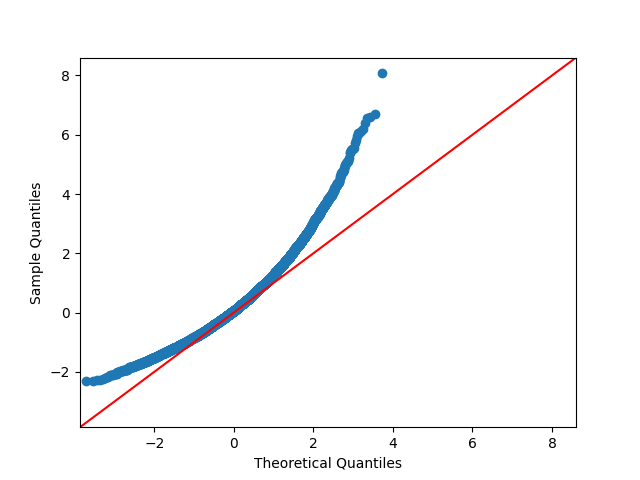
\includegraphics[scale=0.5]{Z6_4_2b} 
\end{center}

\begin{center}
$n=20,\theta=2$
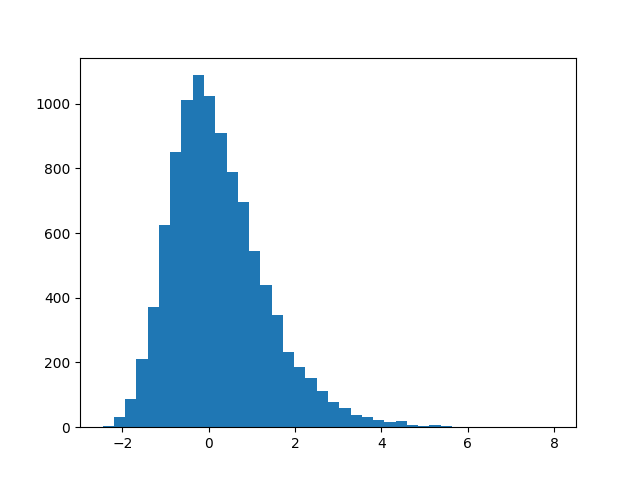
\includegraphics[scale=0.5]{Z6_4_3a}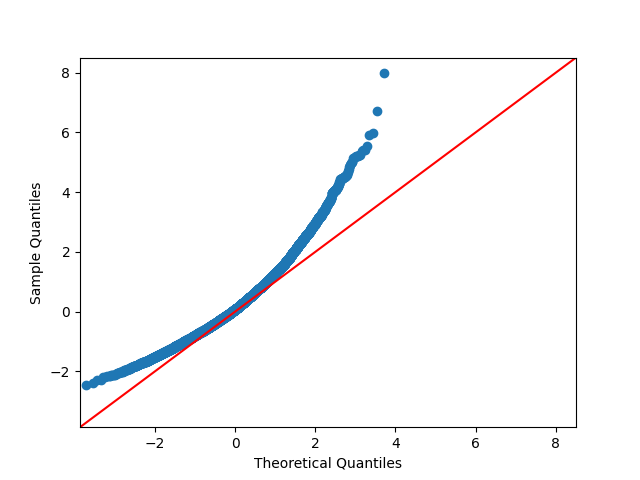
\includegraphics[scale=0.5]{Z6_4_3b} 
\end{center}

\begin{center}
$n=20,\theta=5$
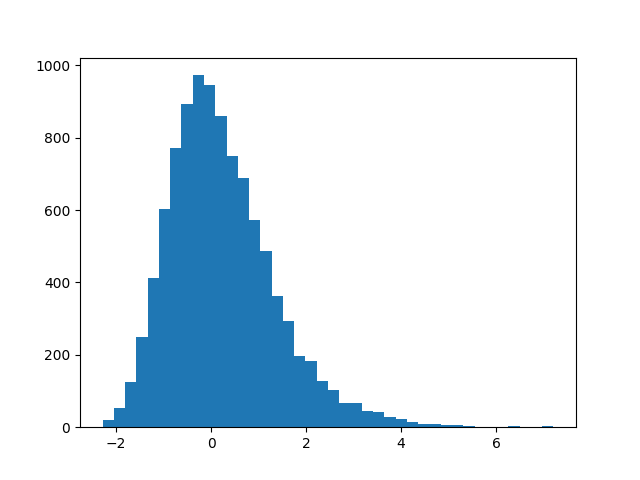
\includegraphics[scale=0.5]{Z6_4_4a}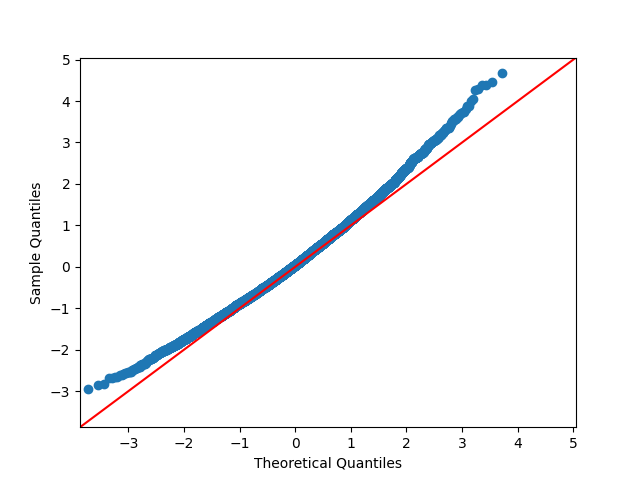
\includegraphics[scale=0.5]{Z6_4_4bb} 
\end{center}
\newpage

\begin{center}
$n=100,\theta=0.5$
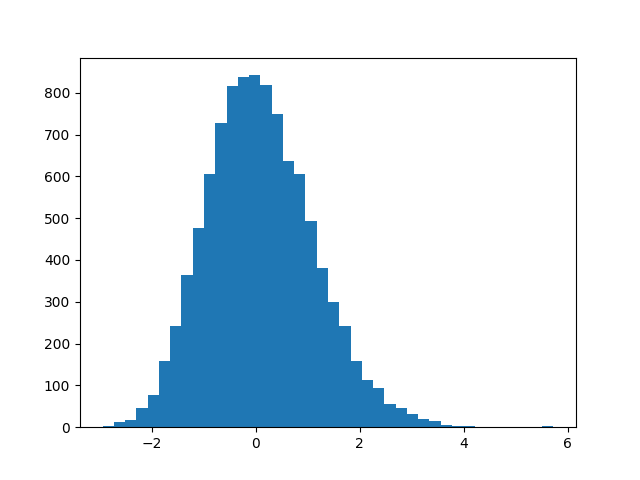
\includegraphics[scale=0.5]{Z6_4_1aa}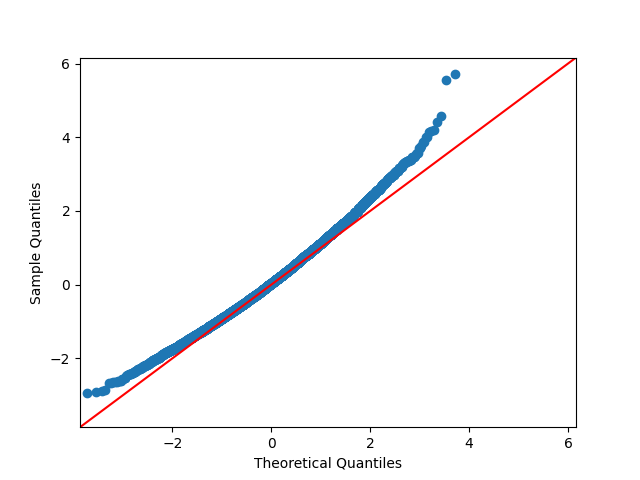
\includegraphics[scale=0.5]{Z6_4_1bb} 
\end{center}


\begin{center}
$n=100,\theta=1$
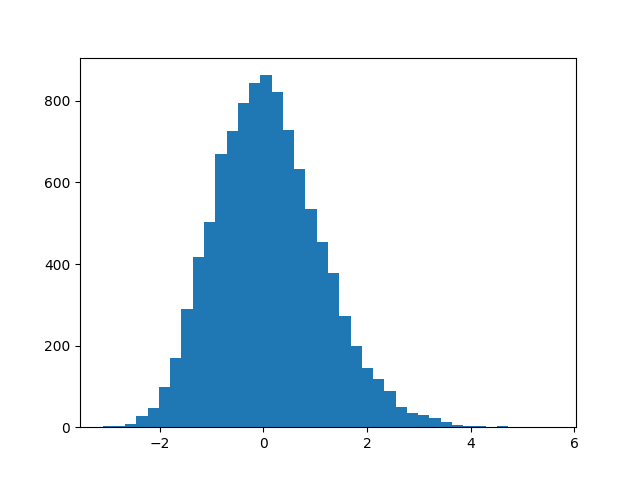
\includegraphics[scale=0.5]{Z6_4_2aa}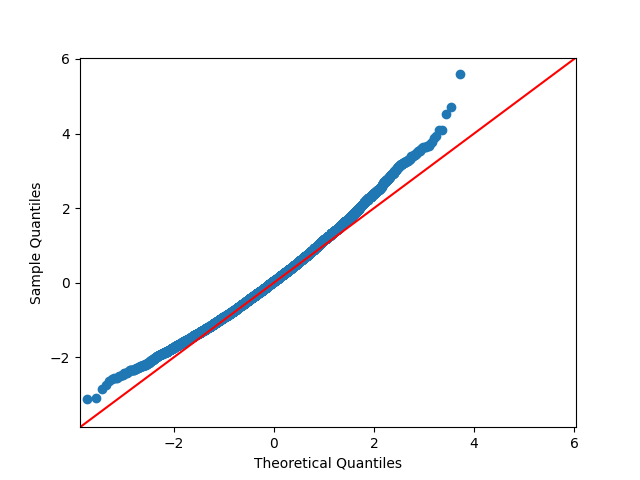
\includegraphics[scale=0.5]{Z6_4_2bb} 
\end{center}

\begin{center}
$n=100,\theta=2$
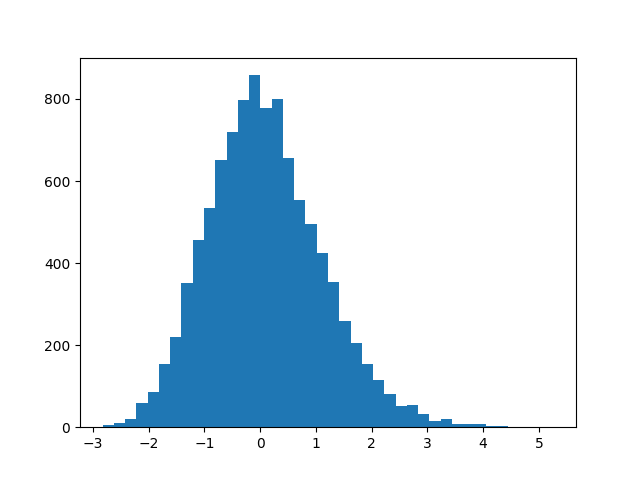
\includegraphics[scale=0.5]{Z6_4_3aa}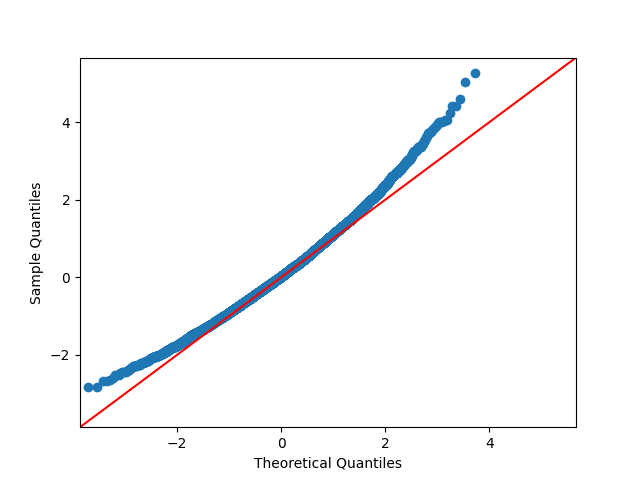
\includegraphics[scale=0.5]{Z6_4_3bb} 
\end{center}
\newpage

\begin{center}
$n=100,\theta=5$
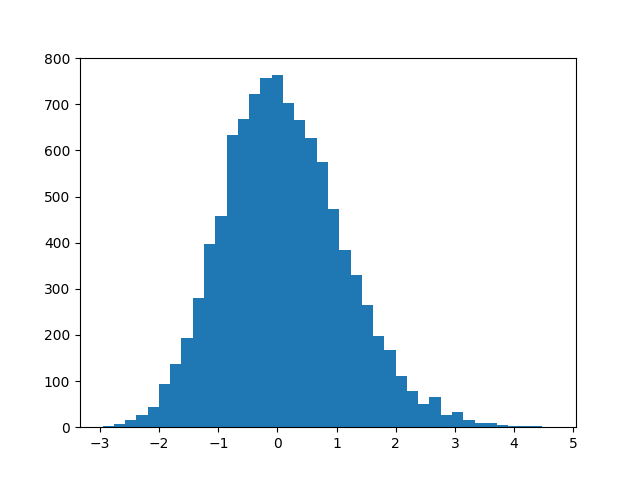
\includegraphics[scale=0.5]{Z6_4_4aa}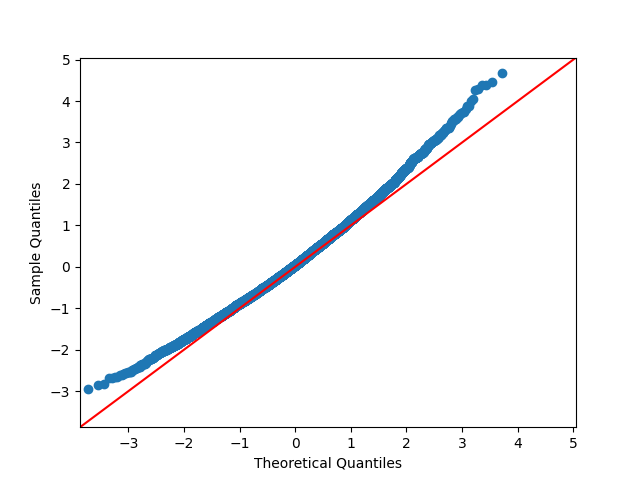
\includegraphics[scale=0.5]{Z6_4_4bb} 
\end{center}

Wykresy obrazują powolną zbieżność do rozkładu normalnego wraz ze zwiększaniem $n$.
\newline

\textbf{Zadanie 5.}



\begin{table}[H]
\centering
\begin{tabular}{|c|c|c|c|}
\hline
\multicolumn{4}{|c|}{$n=20$, $\theta=1$, $\sigma=1$} \\ \hline
                  & \textbf{wariancja}   & \textbf{błąd średniokwadratowy} & \textbf{obciążenie estymatora} \\ \hline
$\hat{\theta}_1$ & 0.03875034 & 0.03875415 & 0.00195064 \\ \hline
$\hat{\theta}_2$ & 0.02344509 & 0.02344669 & 0.00126500 \\ \hline
$\hat{\theta}_3$ & 0.05080761 & 0.05081367 & 0.00246120 \\ \hline
$\hat{\theta}_4$ & 0.04035669 & 0.15400074 & 0.33711132 \\ \hline
\multicolumn{4}{|c|}{$n=20$, $\theta=4$, $\sigma=1$} \\ \hline
                  & \textbf{wariancja}   & \textbf{błąd średniokwadratowy} & \textbf{obciążenie estymatora} \\ \hline
$\hat{\theta}_1$ & 0.04056163 & 0.04058679 & 0.00501553 \\ \hline
$\hat{\theta}_2$ & 0.02430033 & 0.02430494 & 0.00214645 \\ \hline
$\hat{\theta}_3$ & 0.05324878 & 0.05325972 & 0.00330787 \\ \hline
$\hat{\theta}_4$ & 0.03932861 & 7.14692468 & 2.66600751 \\ \hline
\multicolumn{4}{|c|}{$n=20$, $\theta=1$, $\sigma=2$} \\ \hline
                  & \textbf{wariancja}   & \textbf{błąd średniokwadratowy} & \textbf{obciążenie estymatora} \\ \hline
$\hat{\theta}_1$ & 0.16354358 & 0.16356740 & 0.00488048 \\ \hline
$\hat{\theta}_2$ & 0.10020293 & 0.10020897 & 0.00245707 \\ \hline
$\hat{\theta}_3$ & 0.21412813 & 0.21415132 & 0.00481537 \\ \hline
$\hat{\theta}_4$ & 0.15692464 & 2.95880933 & 1.67388311 \\ \hline
\end{tabular}
\end{table}



\begin{table}[H]
\centering
\begin{tabular}{|c|c|c|c|}
\hline
\multicolumn{4}{|c|}{$n=100$, $\theta=1$, $\sigma=1$} \\ \hline
                  & \textbf{wariancja}   & \textbf{błąd średniokwadratowy} & \textbf{obciążenie estymatora} \\ \hline
$\hat{\theta}_1$ & 0.01984403 & 0.01984608 & 0.00143204 \\ \hline
$\hat{\theta}_2$ & 0.01140494 & 0.01140564 & 0.00083562 \\ \hline
$\hat{\theta}_3$ & 0.02648698 & 0.02648727 & 0.00053772 \\ \hline
$\hat{\theta}_4$ & 0.02022635 & 0.15078861 & 0.36133398 \\ \hline
\multicolumn{4}{|c|}{$n=100$, $\theta=4$, $\sigma=1$} \\ \hline
                  & \textbf{wariancja}   & \textbf{błąd średniokwadratowy} & \textbf{obciążenie estymatora} \\ \hline
$\hat{\theta}_1$ & 0.02027044 & 0.02027181 & 0.00116787 \\ \hline
$\hat{\theta}_2$ & 0.01158574 & 0.01158621 & 0.00068363 \\ \hline
$\hat{\theta}_3$ & 0.02714857 & 0.02715159 & 0.00173992 \\ \hline
$\hat{\theta}_4$ & 0.02080980 & 6.98873111 & 2.63968204 \\ \hline
\multicolumn{4}{|c|}{$n=100$, $\theta=1$, $\sigma=2$} \\ \hline
                  & \textbf{wariancja}   & \textbf{błąd średniokwadratowy} & \textbf{obciążenie estymatora} \\ \hline
$\hat{\theta}_1$ & 0.07914722 & 0.07917998 & 0.00572361 \\ \hline
$\hat{\theta}_2$ & 0.04615325 & 0.04618822 & 0.00591339 \\ \hline
$\hat{\theta}_3$ & 0.10535379 & 0.10539758 & 0.00661691 \\ \hline
$\hat{\theta}_4$ & 0.08212816 & 3.04526291 & 1.72137583 \\ \hline
\end{tabular}
\end{table}

Powyższe dane utwierdzają w przekonaniu o tym, że to właśnie mediana jest optymalnym estymatorem $\theta$ w rozkładzie Laplace'a.

\end{document}
